\chapter{Graph Theory}
In this chapter, we will discuss Graph Theory, a highly applicable set of mathematical theories that help with algorithmical operations via representational abstractions in computational and mathematical notions.

\section{An Introduction to Graph Theory}

\subsection{Motivation}
Abstraction. It is the universal theme of many things computer science. We attempt to capture the essence, simple representation of a complex situation, from concepts to functions. \\
And graphs happen to be a very popular abstraction. Graphs are sets of connections between customizable individuals, working from neural networks (individuals are neurons) to your mom (individuals are cells, connections are the chemical interactions of cells). \\
This mathematical object, graphs, have been developed by mathematicians and scientists. Eventually, we are provided a framework for the object, and this framework is known as \textbf{graph theory}.
\begin{ln-define}{Graph Theory}{}
    The mathematical theory of properties and applications of Graphs.
\end{ln-define}
Albeit I realize that grades would be a popular motivation for studying, understanding graphs will provide good fluency across many advanced computational concepts. It is necessary, and is essential to the language of mathematics and computers.

\subsection{Foundations and Formation of Graphs}
Formally, a \textbf{graph} is defined by a set of \textbf{vertices} $V$ and a set of \textbf{edges} $E$. Vertices are the individuals and edges are the connections. \\
Graphically, each vertex corresponds to the small circles in the following example of graphs, while edges are line segments connecting these vertices:
\setbox\codebox=\hbox{
    \begin{lstlisting}
        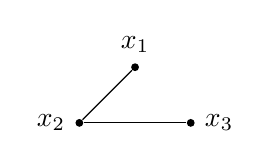
\begin{tikzpicture}
            [point/.style = {circle, fill, inner sep = 1pt}]
            \node[point] (1) [label=above:$x_1$] {};
            \node[point] (2) [below left of=1, label=left:$x_2$] {};
            \node[point] (3) [below right of=1, label=right:$x_3$] {};
            \draw (1) -- (2);
            \draw (2) -- (3);
        \end{tikzpicture}
    \end{lstlisting}
}
\begin{ln-fig}{Example of a Graph}{}
    \begin{center}
        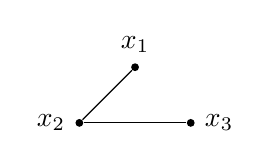
\begin{tikzpicture}
            [point/.style = {circle, fill, inner sep = 1pt}]
            \node[point] (1) [label=above:$x_1$] {};
            \node[point] (2) [below left of=1, label=left:$x_2$] {};
            \node[point] (3) [below right of=1, label=right:$x_3$] {};
            \draw (1) -- (2);
            \draw (2) -- (3);
        \end{tikzpicture}
    \end{center}
    \tcblower
    The $LaTeX$ code is shown as follows: \\
    \usebox\codebox
\end{ln-fig}

\begin{ln-think}{How do you mathematically represent the graph in Figure 5.1.1?}{}
    The set of its vertices would be $V = \{x_1, x_2, x_3\}$. \\
    Its edge, meanwhile, can be contained in the set $E = {{x_1, x_2}, {x_2, x_3}}$
\end{ln-think}
Notice that here, $E$ is a multiset, meaning there can be an element appearing multiple times if an edge is repeated. But we would really like $E$ to be a set instead. \\
To let repeated edges that might have had different directions be counted distinctly, let us also define a directed graph, where each edge must have a direction:
\setbox\codebox=\hbox{
    \begin{lstlisting}
        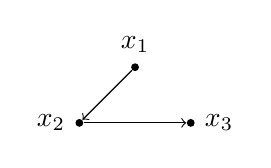
\begin{tikzpicture}
            [point/.style = {circle, fill, inner sep = 1pt}]
            \node[point] (1) [label=above:$x_1$] {};
            \node[point] (2) [below left of=1, label=left:$x_2$] {};
            \node[point] (3) [below right of=1, label=right:$x_3$] {};
            \draw[->] (1) -- (2);
            \draw[->] (2) -- (3);
        \end{tikzpicture}
    \end{lstlisting}
}
\begin{ln-fig}{Example of a Graph}{}
    \begin{center}
        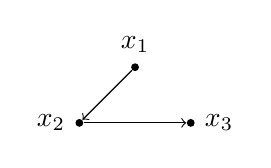
\begin{tikzpicture}
            [point/.style = {circle, fill, inner sep = 1pt}]
            \node[point] (1) [label=above:$x_1$] {};
            \node[point] (2) [below left of=1, label=left:$x_2$] {};
            \node[point] (3) [below right of=1, label=right:$x_3$] {};
            \draw[->] (1) -- (2);
            \draw[->] (2) -- (3);
        \end{tikzpicture}
    \end{center}
    \tcblower
    The $LaTeX$ code is shown as follows: \\
    \usebox\codebox
\end{ln-fig}
The example shown above is known as a \textbf{directed graph}, graphs equipped with directed edge.
\begin{ln-define}{Directed-ness of Edge}{}
    If an edge models a one-way path from one vertex to another, such an edge is known as a \textbf{directed edge}. Mathematically, it is represented as an edge with an arrowmark. \\
    For the edge set \underline{from the above example},
    \[(x_1, x_2) \in E \land (x_2, x_1) \notin E\]
    If an edge is not arrowmarked, such that it allows travel between two vertices in both directions, then the edge is an \textbf{undirected edge}.
\end{ln-define}
We can use a directed edge on multiple abstractions. For example, in a circuit diagram, current flows from one point to another in a single direction. \\
But, an undirceted graph is also useful for modeling, say a metro map, where it is free to commute between stations for any direction.

\subsection{Edge and Degree}
For an undirected edge $e = (u, v)$ (or in equivalent notation, $\{u, v\}$), such edge $e$ is said \textbf{incident} on vertices $u$ and $v$. \\
Meanwhile, these vertices connected by a same edge would be neighbors, or in more formal terms, \textbf{adjacent}. If a vertex is involved in no edge, it is called an \textbf{isolated vertex} and would also be disconnected from the graph.\\
A directed graph, however, has one-directional edges. In that case, vertices will still be incident, but the way to calculate visits slightly differs. We will see when we discuss the metric of visit frequency of vertices. \\
We may also use a metric to see how frequently a vertex is involved in the travelings of graphs: \textbf{degree}.
\begin{ln-define}{Degree}{}
    In general, \textbf{degree} measures the amount of edges a vertex has been visited by or involved in. \\
    Such measure would differ slightly in the context of graph: whether it is directed or undirected.

    If the graph is undirected, then degree of a vertex $u$ is calculated as the amount of edges that involve $u$:
    \[deg(u) = |\{v \in V: {u, v} \in E\}|\]

    If the graph is directed, there are thwn two measures of degree:
    \begin{bindenum}
        \item In-degree of $u$: The amount of edges that directs towards $u$.
        \item Out-degree of $u$: The amount of edges that directs from $u$.
    \end{bindenum}
\end{ln-define}
If an edge originates from one vertex to itself, then this edge ${u, u}$ is known as a \textbf{self-loop}. Again, depending on abstraction, this can either be utterly useless information or very useful information. \\
Since it is difficult to analyze graphs with self-loops, we will talk about graphs without self-loops in the following sections, and will not discuss the occassion of multiple edges between a pair of vertices (unless their directions are all distinct).

\subsection{Traversing a Graph, Mathematically}
We traverse graphs, algorithmically most of the time. How do we mathematically characterize a traverse?
\begin{ln-define}{Path}{}
    A \textbf{path} in a graph $G$ is a sequence of edges. A path would, then, start from one vertex and end at a vertex. \\
    Essentially, it is an itinerary, a projectory of traverse! \\
    A path is \textit{simple} when the vertices it travels are distinct.
\end{ln-define}
\begin{ln-define}{Cycle, Tour}{}
    A \textbf{cycle} is a sequence of edges that starts and ends at the same vertex. \\
    More specifically, all vertices traveled are distinct except the starting and ending vertex, and no edges are repeated. \\
    If a sequence of edges simply starts and ends at the same vertex, it is known as a \textbf{tour}.
\end{ln-define}
Let`s make a brief summary:
\begin{ln-fig}{Walk vs Path vs Cycle vs Tour}{}
    \begin{center}
        \begin{tabular}{c||c|c|c}
            Type & No Repeated Vertices & No repeated edges & Start is End \\
            \hline
            \hline
            Walk & & & \\
            \hline
            Path & $\bigcirc$ & $\bigcirc$ & \\
            \hline
            Tour & & & $\bigcirc$ \\
            \hline
            Cycle & except start and end & $\bigcirc$ & $\bigcirc$
        \end{tabular}
    \end{center}
\end{ln-fig}

\subsection{Connectivity}
Previously, we discussed the notion of isolated vertices. How do we, then, mathematically describe the connected-ness of a graph?
\begin{ln-define}{Connectivity}{}
    A graph is \textbf{connected} if there is a path between any two distinct vertices. This means isolated vertex is in fact a connected component. \\
    On the contrary is a \textbf{disconnected} graph.
\end{ln-define}
Let me demonstrate with some examples:
\begin{ln-fig}[sidebyside]{Connected vs Disconnected}{}
    \begin{center}
        \textbf{Disconnected}: \\

        \vspace{0.2cm}
        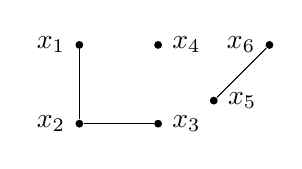
\begin{tikzpicture}
            [point/.style = {circle, fill, inner sep = 1pt}]
            \node[point] (1) [label=left:$x_1$] {};
            \node[point] (2) [below of=1, label=left:$x_2$] {};
            \node[point] (3) [right of=2, label=right:$x_3$] {};
            \node[point] (4) [above of=3, label=right:$x_4$] {};
            \node[point] (5) [below right of=4, label=right:$x_5$] {};
            \node[point] (6) [above right of=5, label=left:$x_6$] {};
            \draw (1) -- (2);
            \draw (2) -- (3);
            \draw (5) -- (6);
        \end{tikzpicture}
    \end{center}
    As you may have seen, vertex $4$ is an isolated vertex that no one visits (just like me). \\
    Meanwhile, the subgraph involving vertex $5$ and $6$ is disconnected from the rest of the graph, as well as the isolated vertex. 
    \tcblower
    \begin{center}
        \textbf{Connected}:
        
        \vspace{0.2cm}
        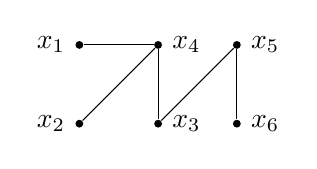
\begin{tikzpicture}
            [point/.style = {circle, fill, inner sep = 1pt}]
            \node[point] (1) [label=left:$x_1$] {};
            \node[point] (2) [below of=1, label=left:$x_2$] {};
            \node[point] (3) [right of=2, label=right:$x_3$] {};
            \node[point] (4) [above of=3, label=right:$x_4$] {};
            \node[point] (5) [right of=4, label=right:$x_5$] {};
            \node[point] (6) [right of=3, label=right:$x_6$] {};
            \draw (1) -- (4);
            \draw (2) -- (4);
            \draw (3) -- (4);
            \draw (3) -- (5);
            \draw (5) -- (6);
        \end{tikzpicture}
    \end{center}
    In such a connected graph, there is a path from every vertex to another vertex.
    \\
    \\
    \\
\end{ln-fig}

\section{Koenigsberg`s Seven Bridges and Eulerian Tour}

\subsection{The Seven Bridges of Koenigsberg}
Imagine that there are seven bridges connecting four cities, abstractable to the graph as seen below:
\begin{ln-fig}{Seven Bridges of Koenigsberg}{}
    The Seven Bridges of Koenigsberg can be represented by the graph as follows:
    \begin{center}
        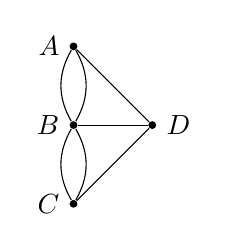
\begin{tikzpicture}
            [point/.style = {circle, fill, inner sep = 1pt}]
            \node[point] (B) [label=left:$B$] {};
            \node[point] (A) [above of=B, label=left:$A$] {};
            \node[point] (C) [right of=B, label=right:$D$] {};
            \node[point] (D) [below of=B, label=left:$C$] {};
            \draw (A) edge[bend left] (B) {};
            \draw (A) edge[bend right] (B) {};
            \draw (D) edge[bend left] (B) {};
            \draw (D) edge[bend right] (B) {};
            \draw (A) -- (C);
            \draw (B) -- (C);
            \draw (D) -- (C);
        \end{tikzpicture}
    \end{center}
    Where the seven edges each are distinct bridges, and the four vertices are distinct cities.
\end{ln-fig}
Now, the question is: is there a route that would traverse each seven bridges precisely once and return to the starting point.

\subsection{Euler`s Take}
Euler, having contributed a lot to graph theory, came with some terminologies regarding itineraries of traversals:
\begin{ln-define}{Eulerian Itineraries}{}
    \textbf{Eulerian Walk} is a walk of graph $G$ that uses each of its edge exactly once. \\
    \textbf{Eulerian Tour} is a closed Eulerian walk where the starting and ending point are the same vertex.
\end{ln-define}
This rephrases the Seven Bridge Problem to: ''Is there an Eulerian tour for its representative graph?'' \\
The answer lies in the Eulerian Theorem:
\begin{ln-theorem}{Eulerian Theorem}{}
    An undirected graph $G = (V, E)$ has an Eulerian tour iff G is even degree, and connected (except isolated vertices). \\
    An \textbf{even-degreed} graph is a graph where all vertices have even degree.
\end{ln-theorem}
Its proof is as follows:
\begin{ln-think}{Prove the Eulerian Theorem!}{}
    \textbf{Proving the forward direction of theorem}: \\
    Assume $G$ has an Eulerian tour. Since it has to use every single edge, every vertex that has an adjacent edge will be involved in this tour, therefore connected with all other vertices on the tour. \\
    Meanwhile, because everytime a tour enters a vertex along an edge, it exits along a different edge, each vertex will have a pair of edge adjacent to it. The start vertex would also have the same phenomenon, since we begin from and end at the starting vertex. \\
    In that case, the graph would be even-degreed for the pairs of edge that occurs on vertices (which must all be used up), and would be connected. \\
    \textbf{Proving the backward direction of theorem}: \\
    Let us first have a subroutine called FIND\_TOUR that finds a tour from a graph $G$. \\
    Notice that while the tour is not necessarily Eulerian, it must get stuck at the vertex it started at, because it would then deplete the pairs of edges it can continue its travel with. This does not serve as a formal proof, but hopefully the conceptual summary of lecture notes' claim is good enough. \\
    Then, let`s also involve another subroutine SPLICE, which outputs a single tour $T'$ provided a tour $T$ that intersects each of the other arguments $T_1, \dots, T_i$. Last but not least, these tours are merged together. The input tours are all edge-disjoint. \\
    Last but not least, EULER, which once provided a graph $G$ and starting vertex $s$, will attempt to find a spliced tours $G_1, \dots, G_i$ from an arbitrary found tour $T$ of $EULER(G_i, s)$, and its edge-disjoint intersected tours. \\
    Let us use a shortened mathematical induction to prove the functionality of EULER: \\
    \begin{bindenum}
        \item[] {
            \textbf{Base Case}: \\
            The graph has 0 edges, there is no tour to find.
        }
        \item[] {
            \textbf{Induction Hypothesis}: \\
            EULER outputs an Eulerian Tour for any even degree, connected graph with at most $m \geq 0$ edges. This is a strong induction!
        }
        \item[] {
            \textbf{Induction Step}: \\
            Suppose $G$ has $m + 1$ edges. Removing the edges of $T$ from $G$, since the tour would remove pairs of edges from vertices, we would be left with a remaining even-degree, connected graph with less than $m$ edges. \\
            This $T$ intersects each of the edge disjointed but connected subtours $G_i$, at some first vertex of intersection. \\
            The induction hypothesis allows us to assume these resultant subtours to have Eulerian tours. Therefore, our end result of EULER is in fact a splice of individual Eulerian tours, into a large tour whose union is all edges of $G$ and thus also an Eulerian tour.
        }
    \end{bindenum}
    Such is the general description of this proof.
\end{ln-think}
In this case, since the graph of Seven Bridge is not even-degreed, it cannot have an Eulerian Path. Therefore, the solution is impossible.

\section{Planarity, Euler`s Formula, Coloring}

\subsection{Trees}
Trees are defined as connected acyclic graphs, with some interesting properties upon observation:

\begin{bindenum}
    \item On a tree, any node can be set as a root.
    \item Any degree-1 node on a tree would be called a ``leaf'' node.
    \item A tree is in fact bipartite. We will talk about this later.
    \item A tree is always planar. We will talk about this later.
    \item Adding an edge to anywhere of a tree will make it cyclic.
\end{bindenum}

\subsection{Planar Graphs}
What is a planar graph?
\begin{ln-define}{Planarity}{}
    A graph is planar if it can be drawn on a plane without crossings.
\end{ln-define}
In that case, all trees are planar. \\
\begin{ln-symbol}{Three Houses-Three Wells}{}
    The graph $K_{3,3}$ is a graph where there are two sets of vertices, each of size three, and all edges between the two sets of vertices are present:
    \begin{center}
        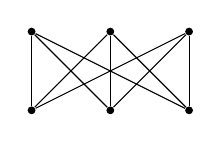
\begin{tikzpicture}
            [point/.style = {circle, fill, inner sep = 1pt}]
            \node[point] (A) [] {};
            \node[point] (B) [right of=A] {};
            \node[point] (C) [right of=B] {};
            \node[point] (D) [below of=A] {};
            \node[point] (E) [right of=D] {};
            \node[point] (F) [right of=E] {};
            \draw (A) -- (D);
            \draw (A) -- (E);
            \draw (A) -- (F);
            \draw (B) -- (D);
            \draw (B) -- (E);
            \draw (B) -- (F);
            \draw (C) -- (D);
            \draw (C) -- (E);
            \draw (C) -- (F);
        \end{tikzpicture}
    \end{center}
\end{ln-symbol}
Shown in above is an example of a nonplanar graph, $K_{3,3}$. \\
Another example of a nonplanar graph would be a complete graph with five nodes, notated as $K_5$. A complete graph is a graph where every possible edge is present. \\
And from here, let us introduce another useful notion in the discussion of graphs by its edges:
\begin{ln-define}{Bipartite Graphs}{}
    A bipartite graph, $G = (V, E)$, is a graph where vertices are split into two groups and edges only exist between groups. \\
    Mathematically, let the groups of vertices be $L$, $R$, then $V = L \cup R$ and $E \subseteq L \times R$.
\end{ln-define}

\subsection{Euler`s Formula}
Planar graphs, when drawn on the plane, separates a plane into multiple regions. How do we express this fact mathematically?
\begin{ln-define}{Faces}{}
    The faces of a graph are the regions which the graph subdivides the plane into. \\
    Faces are distinguishable for a planar graph, but not much so for nonplanar graphs!
\end{ln-define}
Euler has contributed a great formula for planar graphs, which are great generalizations of polyhedra.
\begin{ln-theorem}{Euler`s Formula}{}
    Let $v$, $f$, $e$ be respectively the amount of vertices, faces, and edges in a connected planar graph. \\
    Then, $v + f = e + 2$.
\end{ln-theorem}
And let`s proceed with a proof:
\begin{ln-quest}{Prove Euler`s Formula}{}
    We can perform mathematical induction on value of $e$. \\
    \textbf{Base Case} $e = 0$:\\
    In this case, since there is no edge, the amount of vertex and face are all $1$. The formula holds. \\
    \textbf{Induction Hypothesis} For all connected planar graphs, the prompt holds. \\
    \textbf{Induction Step} Let`s consider the following cases:
    \begin{itemize}
        \item If it is a tree, then the amount of faces is $1$ and the amount of edge $e$ in a tree is equal to $v - 1$.
        \item If it is not a tree, find a cycle of the graph and delete any edge of the cycle to break it. This will reduce both $e$ and $f$ by one. By induction hypothesis, formulas work in the smaller graph, and the arithmetics we just performed would prove the formula true in a graph with $e - 1 + 1 = e$ edges.
    \end{itemize}
\end{ln-quest}
For a non-connected planar graph, the situation is slightly different.
\begin{ln-theorem}{The Sparsity of Graph}{}
    Take its connected subpart, a planar graph that has $f > 1$ faces, and count the number of sides on each face. In the end, as we double count each side, we double count each edge of the graph, resulting in the conclusion:
    \[\sum_{i = 1}^f (\text{Number of sides in face $i$}) = 2e\]
    Knowing that there cannot be parallel edges between two same nodes, and assuming that the graph has at least two edges (to secure at least three vertices), then each face has at least three sides. \\
    \begin{align*}
        \text{Number of sides in face $i$} &\geq 3 \\
        \sum_{i = 1}^f 3 &\leq \sum_{i = 1}^f (\text{Number of sides in face $i$}) = 2e
    \end{align*}
    Since we are considering a connected planar graph, let us transform the above inequality according to Euler`s Formula:
    \begin{align*}
        2e &\geq 3f \\
        2e &\geq 3(e + 2 - v) \\
        2e &\geq 3e - 3v + 6 \\
        e &\leq 3v - 6
    \end{align*}
\end{ln-theorem}
This implies that planar graphs are sparse, or, they cannot have too many edges. \\
Therefore, specific graphs whose number of edges and vertices do not follow the above inequality can be seen as non-planar:
\begin{ln-define}{Planarity}{}
    If a graph is a connected planar graph, $e \leq 3v - 6$. \\
    Mind that this does not serve as a planarity test, as such property is satisfied by $K_{3, 3}$ as well. \\
    However, its contrapositive can serve as a non-planarity test.
\end{ln-define}
In that case, both $K_5$ and $K_{3,3}$ are non-planar. We can explore these graphs further: these are the only non-planar graphs, made precise by the mathematician Kuratowski (where the capital K came from).
\begin{ln-theorem}{Kuratowski's Theorem}{}
    A graph is non-planar iff it contains $K_5$ or $K_{3,3}$.
    \tcblower
    Let us define contain as where the nodes in the graph $K_5$ or $K_{3,3}$ are identifiably connected as their corresponding graph rules via paths, such that no two of those paths share vertices. \\
    In otherwords, let the graphs noted in this theorem be a subgraph of the larger inspected graph. \\
    This mathematical result is sometimes also known as Kuratowski`s theorem, and its direction imply that if a graph contains one of these two non-planar graphs, itself must also be non-planar.
\end{ln-theorem}

\subsection{Duality and Coloring}
The Greeks knew everything, from the section above to the next notion:
\begin{ln-define}{Dual Graph}{}
    The dual graph $G*$ of a graph $G$ is a graph formed by converting faces of $G$ into vertices and drawing edges between adjacent faces.
\end{ln-define}
And the CS70 Lecture Note will ask you to \textit{think about it :::::D}. So do it, maybe search a few Google Images up. I can't LaTeX this. Skill issue. \\
But Brandon, \textbf{I hear your thoughts}. Why did you put a LaTeX-ized dual graph on the screen already
\begin{ln-fig}{Dual Graph}{}
    \begin{center}
        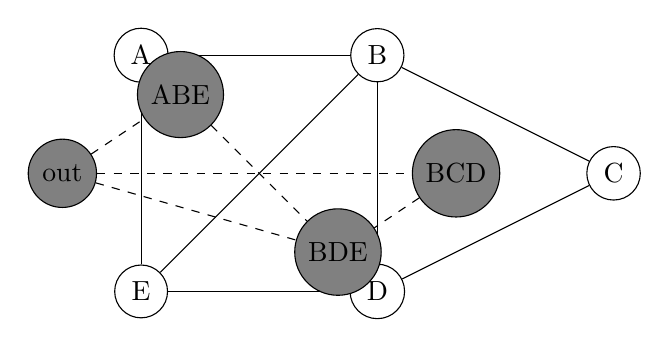
\begin{tikzpicture}
            [
                main/.style = {draw, circle}
            ] 
            \node[main] (A) at (0, 3) {A};
            \node[main] (B) at (3, 3) {B};
            \node[main] (C) at (6, 1.5) {C};
            \node[main] (D) at (3, 0) {D};
            \node[main] (E) at (0, 0) {E};
            \draw (A) -- (B);
            \draw (B) -- (C);
            \draw (B) -- (D);
            \draw (B) -- (E);
            \draw (C) -- (D);
            \draw (D) -- (E);
            \draw (E) -- (A);
            \begin{scope}[main/.style = {draw, circle, fill=gray}]
                \node[main] (ABE) at (0.5, 2.5) {ABE};
                \node[main] (BDE) at (2.5, 0.5) {BDE};
                \node[main] (BCD) at (4, 1.5) {BCD};
                \node[main] (out) at (-1, 1.5) {out};
            \end{scope}
            \draw[dashed] (out) -- (ABE);
            \draw[dashed] (out) -- (BDE);
            \draw[dashed] (out) -- (BCD);
            \draw[dashed] (ABE) -- (BDE);
            \draw[dashed] (BCD) -- (BDE);
        \end{tikzpicture}
    \end{center}
\end{ln-fig}
and why is Duality important at all? \\
That's because it reduces area-coloring map into a planar graph. Since a map's faces ought to be distinguishable, its dual graph can serve as a planar graph for us to work with. \\
Now let's talk about coloring. Essentially, two-coloring a graph is working with a bipartite graph, where one group of vertex has one specific color, the other group the other color. \\
Or, we may proceed with a breadth-first algorithm that colors any uncolored neighbor with alternative colors. This will let us discover cycles of odd lengths in the event of failing to color.

Notably, we have the four color theorem, which states that you may graph any map with four colors. This implies that any planar graph can be vertex-colored in four or more colors!

Furthermore, there are in fact two types of coloring: vertex coloring and edge coloring. \\
To color a graph by some component $X$ means all adjacent components of type $X$ must not have a same color.

\section{Classes of Graphs}

\subsection{Complete Graphs}
Starting with a definition,
\begin{ln-define}{Complete Graph}{}
    A complete graph contains all possible edges between its vertices. \\
    A complete graph on $n$ vertex is unique and denoted as $K_n$, and has $\frac{n(n-1)}{2} $edges.
\end{ln-define}

\subsection{Trees}
Starting with a definition$\dots$ well, in fact, many definitions.
\begin{ln-define}{Trees}{}
    Trees can be defined as any of the following:
    \begin{bindenum}
        \item A graph that is connected and acyclic (as spoken in last section).
        \item A graph that is connected and has $n - 1$ edges (this guarantees it to be acyclic).
        \item A graph that is connected, and the removal of an arbitrary edge disconnects the graph.
        \item An acyclic graph that becomes cyclic upon the addition of edge on any possible position.
    \end{bindenum}
\end{ln-define}
Why do we want trees? I don't know, maybe retaking CS61B will provide you some insights.

In a rooted trees, which algorithms are mainly concerned with, there is a designated node called the root at the topmost level of a tree. The bottom-most nodes are called leaves, and the intermediate nodes are called internal nodes. \\
In a rooted tree, a root should never be a leaf; and throughout types of trees, leaves ought to be degree-1 vertices. \\
But why does this matter? That's a nice question. James. I have been tested on this when practicing Leetcode. I think that shows something.

\subsection{Hypercubes}
We would like a graph to be strongly connected, and a complete graph is such example. But, complete graphs take a lot, a lot of edges. Since graphs are abstractions of real-life objects, this implies huge operational and development costs. Our alternative solution would be a hypercube.
\begin{ln-define}{Hypercube}{}
    A hypercube is a graph whose vertex set is given by:
    \[V = {\{0, 1\}}^n\]
    which is equivalent of the set of all n-bit strings. \\
    The edge set is then defined as:
    \[E = \{{x, y}: \text{x and y differ in one bit}\}\]
    Such a hypercube is also called an n-dimensional hypercube.
\end{ln-define}
Notably, we may deifne hypercube recursively. \\
The vertex set of a $n - 1$ dimensional hypercube happens to be $\{0x | x \in V_{n - 1}\}$. The $n$-dimensional hypercube is obtained by placing an edge between each pair of vertices in the 0-subcube, which we described via an $n - 1$ dimensional hypercube, and the 1-subcube where every leftmost digit of such vertex group is $1$ instead! \\
Well, let's take a further investigation into its connectivity, so to make sure that we are working with the alternative solution we have wanted:
\begin{ln-lemma}{Total Number of Edges in Hypercube}{}
    By the definition of hypercube, $E(n)=2E(n-1)+2^{n-1}$, where $E(1)=1$. \\
    Using mathematical induction, we may show that $E(n) = n2^{n-1}$.

    In a simpler approach, since the degree of each vertex is $n$ and $n$ bit positions can be flipped in any of the $2^n$ vertices, there is a total of $n 2^n$ edges (non-disticnt) that we can count between cubes. \\
    We counted each edge twice, so we divide that total number by $2$ to attain the result that the total number of edges in a $n$-dimensional hypercube is still $n 2^{n-1}$.
\end{ln-lemma}
\begin{ln-theorem}{The number of discarded edges from disconnected vertices}{}
    Let $S \subseteq V$ such that $|S| \leq |V - S|$, and let $E_S$ denote the set of edges connecting $S$ to $V - S$:
    \[E_S := \{\{u, v\} \in E : u \in S \land v \in (V - S)\}\]
    Then, it must be that $|S| \leq |E_S|$.
\end{ln-theorem}
\begin{ln-quest}{Prove the above theorem}{}
    Let is perform mathematical induction on the dimension of hypercube. \\
    \textbf{Base Case}: $n = 1$ \\
    We may only separate $1$-dimensional hypercubes into one vertex and another. Either way, there will be only one edge connecting $S$ and $V - S$, and the cardinality of such two sets would be $1$. Theorem holds. \\
    \textbf{Induction Hypothesis}: Assume claim holds for $1 \leq n \leq k$; we perform strong induction. \\
    \textbf{Induction Step}: Prove the claim for $n = k + 1$. \\
    Let us assume that among the two separated sets, it would be $|S| \leq 2^k$. \\
    Let $S_0$ represent the vertices from $0$-subcube in $S$, and respectively for $S_1$. Then, either $S$ has a fairly eqaul intersection size with the two subcubes, or it does not. \\
    \textit{Case 1: $|S_0| \leq 2^{k - 1} \land |S_1| \leq 2^{k - 1}$} \\
    The induction hypothesis works on both subcubes, which means there are at least $|S_0|$ edges between $S_0$ and its complement, and similarly for $|S_1|$ and $S_1$. If so, the total number of edges between $S$ and $V - S$ would be at least $|S_0| + |S_1| = |S|$, as the theorem attempts to claim. \\
    \textit{Case 2: $|S_0| \geq 2^{k - 1}$} \\
    In this case, we cannot apply the induction hypothesis as wanted before on the $0$-subcube, but only on the $1$-subcube. But we can apply this onto $|V_0 - S_0|$ instead and infer the amount of edges between them is at least $2^k - |S_0|$. The current total of edges is calculated as $2^k - |S_0| + |S_1|$. \\
    The edges that cross between the $0$-subcubes and $1$-subcubes would be at least $|S_0| - |S_1|$ because there is an edge between every pair of vertices ($0x$, $1x$). Therefore, finally, the number of edges crossing is indeed \underline{at least} $2^k \geq |S|$ as desired. \\
    (The $|S_0| - |S_1|$ was derived from the cardinality of complement from $\{x : \overline{0x} \in S_0\} - \{x : \overline{1x} \in S_1\}$).
\end{ln-quest}

\section{Personal Regard on This Topic}
This is probably the most abstract topic you'll encounter in CS70, just because everyone is new to graphs. \\
Here is also an organization of results we have proven during discussion and homework:
\begin{bindenum}
    \item Every even-degreed connected graph has an Eulerian Tour, a tour on which every edge is used. (Eulerian Theorem)
    \item If a graph contains $K_{3,3}$ or $K_5$, it is non-planar. (Kuratowski)
    \item For a connected planar graph, $v + f = e + 2$. (Euler's Formula)
    \item For a connected planar graph, $e \leq 3v - 6$. This inequality is even tighter on disconnected planar graphs. (Proven in Lecture)
    \item Every planar graph can be vertex-colored with four colors. (Four Color Theorem)
    \item Hypercubes of $n$ dimension has $n 2^{n - 1}$ edges. (Proven in Lecture)
    \item The number of vertices in an undirected graph with odd-degree is even. (Discussion 2B)
    \item An $n$-dimensional hypercube can be edge-colored with $n$ colors. (Discussion 3A)
    \item Every hypercube is bipartite. (Discussion 3A)
    \item A Hamiltonian Tour is a tour where each vertex appears only once, each pair of consecutive vertices are connected by an edge, and the first and last vertex of this path are connected by an edge. (Definition)
\end{bindenum}
